\cotefile{68}
\scanpage{2}
% archive foliation: 1
\textcircled{1.} Jeu (de position)

\textcircled{a} $\left\{\begin{array}{l} C\text{ ensemble des positions }(\unsure{i.e.|:=}\text{ configurations})\\ R\subset C\times C\quad\text{relation}\end{array}\right.$
$((x,y)\in R$ se lit $y\in R(x)$ ou $y$ \uline{successeur} de $x)$.

\inserted{\uline{Déf} Position $x$ terminale $\Longleftrightarrow R(x)=\varnothing$
\[
C_0=\{x\in C\mid R(x)=\varnothing\}=\text{ens des positions terminales}
\]}
% The blue bracket and long return arrow attach this definition after (a).

\textcircled{b} $\left\{\begin{array}{l}J\text{ ensemble des joueurs}\\ i:\inserted{C\setminus}C_{\inserted{0}}\longrightarrow J\end{array}\right.$
$i(x)\longrightarrow$ le joueur qui a l'initiative dans la position $x$
\[
\inserted{C\setminus}C_{\inserted{0}}=\coprod_{j\in J}C(j)
\]
\margin{\uline{NB} \deleted{$i$ \uline{\unsure{n'intervient|n'intéresse} que} \uline{pour $x$ situé sur} $C\setminus C_0$} \deleted{\unsure{J}}}

\textcircled{c} $J\longrightarrow\mathcal P(C_0)\qquad j\longmapsto G_0(j)\subset C_0$
\begin{center}positions terminales \uline{gagnantes} \uline{pour $j$}\end{center}
\margin{\uline{NB} On ne \unsure{suppose pas} $G_0(j)\subset C_0(j)$}

\textcircled{2.} \uline{Parties}.
\deleted{\unsure{2a}} (Ne dépend que de $(C,R)$\ldots)

\uline{Partie} \inserted{(à $n$ coups, $n\in\mathbb N$)}
\[
(x_0,x_1,\ldots,x_n)\in C^{n+1}\qquad \forall\,0\leq i\leq n-1,\quad x_{i+1}\in R(x_i)
\]
\uline{Prolongement} de parties

\uline{Partie terminée} ($\Leftrightarrow$ partie maximale) : telles que $x_n\in C_0$

Partie infinie, partie circulaire. $(x_0,x_1\ldots,x_n)\quad x_n=x_0\quad(n\geq1)$

\uline{Prop} S'il existe une partie circulaire, existe une partie infinie. L'inverse est vrai si $C$ est fini.

\uline{Construction} récurrente
\inserted{\[
C_{-1}=\varnothing\qquad C_0=\{x\in C\mid\forall y\in R(x),\ y\in C_{-1}\}=\{x\in C\mid R(x)=\varnothing\}
\]}
\[
C_1=\{x\in C\mid\forall y\in R(x),\ y\in C_0\}\qquad\text{NB }C_1\supset C_0
\]
\[
\unsure{--}
\]
\[
C_i=\{x\in C\mid\forall y\in R(x),\ y\in C_{i-1}\}
\]
\uline{Prop} $(C_i)$ \unsure{est} \unsure{suite} croiss. d'ensembles.
\[
C_i=\{x\in C\mid\text{tte partie }\deleted{\unsure{commençant}}\inserted{\text{issue de}}\ x\text{ est de longueur }\leq i\}
\]
\uline{Cor} Soit $C_\infty=\bigcup C_i$. Alors
\[
C_\infty=\{x\in C\mid\text{l'ens des }\inserted{\uline{longueurs des}}\text{ parties partant de }x\text{ est borné}\}
\]
\scanpage{3}
% archive foliation: 2
\uline{Cor} Conditions équivalentes

 a) $C=C_\infty$ i.e. pour $\forall x\in C$, l'ens des longueurs des parties partant de $x$ est fini.

 b) $\exists\ C\xrightarrow{l}\mathbb N$ tel que si $y\in R(x)$, on ait $l(y)<l(x)$

[Alors $\forall x\in C$, si $l=l(x)$, on a $x\in C_l$]

\deleted{\unsure{Impl.}}

\uline{NB} Ces conditions impliquent que $\nexists$ partie infinie.
\deleted{Mais} Si $C$ est \deleted{\unsure{in}}fini, \deleted{\unsure{l'inverse est vrai}}\inserted{la réciproque est vraie} : en effet, tte partie \deleted{\unsure{est finie}}\inserted{a alors une longueur} \unsure{au plus} $(\operatorname{card}C)-1=N-1$, i.e. $C=C_{N-1}$

\deleted{\uline{Prop} Si $C$}

\textcircled{3} \uline{Stratégie pour $j\in J$}
\[
\Sigma\subset(C(j)\times C)\cap R\quad\text{tel que}
\]
\[
\forall x\in C(j),\quad\text{on a}\quad(R(x)\ne\varnothing\ (\text{i.e. }x\notin C_0)\Longrightarrow\Sigma(x)\ne\varnothing)
\]
Partie $\underline x=(x_0,\ldots,x_n)$ \uline{compatible} avec stratégie $\Sigma$ pour $j$ :
\[
\forall\,0\leq i\leq n-1\quad\text{tel que }x_i\in C(j),\quad\text{on a }x_{i+1}\in\Sigma(x_i)
\]
\margin{Idem pour \unsure{partie infinie|parties infinies}}

\uline{Stratégie gagnante} \inserted{(pour $j$)} pour $x$ $(\in C)$ :

 a) Toute partie partant de $x$, compatible avec $\Sigma$, est finie

(i.e. $\nexists$ partie infinie partant de $x$, comp. avec $\Sigma$)

 b) \inserted{pour} Toute partie terminée, partant de $x$, \inserted{$(x_0=x,x_1,\ldots,x_n)$} compatible avec $\Sigma$, on a $x_n\in G_0(j)$.

On dit que $x\in C$ est \uline{gagnante} \uline{pour} $j$ si $\exists$ stratégie \deleted{gagnante}\inserted{pour $j$} gagnante pour $x$.
L'ens de ces $x$ est noté $G(j)$

\uline{NB} $G(j)\cap C_0=G_0(j)$

Posons $\overline C(j)=C\setminus C(j)$, $\overline G(j)=C\setminus G(j)$\ldots
\scanpage{4}
% archive foliation: 3
\deleted{\uline{Prop}}\inserted{\uline{Th\unsure{m} 1}}
\[
(C(j)\setminus C_0)\cap G(j)=\{x\in C(j)\inserted{\setminus C_0}\mid\deleted{\unsure{x\in G_0(j)}\ \unsure{\text{ou}}}\ \exists y\in R(x),\ \unsure{\text{avec}}\ y\in G(j)\}
\]
\inserted{$R(x)\cap G(j)\ne\varnothing$}
\[
(\overline C(j)\setminus C_0)\cap G(j)=\{x\in\overline C(j)\mid\forall y\in R(x)\ \text{on a }y\in G(j)\ \deleted{\text{et }\unsure{\text{si}}\ R(x)=\varnothing\ (\text{i.e. }x\in C_0)\ \unsure{\text{alors}}\ x\in G_0(j)}\}
\]
\inserted{$R(x)\subset G(j)$}
\margin{\unsure{S'il n'y a pas} de partie infinie}

\uline{Dém} \deleted{a) Soit $x\in C(j)$}\inserted{$1^\circ)$} Soit $x\in C(j)$, il faut prouver que
\[
x\in G(j)\Longleftrightarrow\deleted{\unsure{x\in G_0(j)\ \text{ou}}}\ \exists y\in R(x),\ y\in G(j).
\]
\deleted{\unsure{x est terminal}}

\deleted{Si $x\in C_0$, c'est clair (cf NB plus haut)}
Soit $x\in C\setminus C_0$ \inserted{i.e. $R(x)\ne0$. Prouvons $\Longrightarrow$ i.e. supposons $x\in G(j)$, prouvons $\exists y$ \unsure{ch}\ldots}, soit $\Sigma$ stratégie \deleted{pour $j$} $x$-gagnante. Considérons $\Sigma(x)$; \unsure{donc} \deleted{nécessairement} $\Sigma(x)\ne\varnothing$, donc $\exists y\in\Sigma(x)$. Je dis que $y\in G(j)$, i.e.

\uline{Lemme} Si $x\in C(j)\cap G(j)$, $\Sigma$ une $j$-stratégie $x$-gagnante, alors $\forall y\in\Sigma(x)$, \inserted{on a} $y\in G(j)$, \inserted{i.e. $\Sigma(x)\subset G(j)$.} Plus précisément $\Sigma$ est aussi $y$-gagnante.

\deleted{En effet, \unsure{parties pour} $\Sigma$}
Trivial sur définitions.

Inversement, supposons $\exists y\in R(x)$ avec $y\in G(j)$, prouvons que $x\in G(j)$. Soit $\Sigma$ une $j$-stratégie $y$-gagnante. On va \inserted{\unsure{en garder|en gardant}} définir une $j$-stratégie \inserted{$\Sigma'$} $x$-gagnante ainsi : Pour $z\in C(j)$, on pose
\[
\Sigma'(z)=\begin{cases}\Sigma(z)\text{ si }z\ne x\\ \{y\}\deleted{\unsure{\text{ou}}}\text{ si }z=x\end{cases}
\]
C'est une $j$-stratégie, car \deleted{si $R(z)\ne\varnothing$ \unsure{-} $R(x)\ne\varnothing$, alors} $\Sigma(z)\ne0$ \deleted{\unsure{pour}} \deleted{(et dans le cas $z\ne x$ pas de pb, mais alors $\Sigma'(z)=\Sigma(z)\ne\varnothing$ par hyp. que $\Sigma$ est stratégie.}

Prouvons que $\Sigma'$ est $x$-gagnante : Soit une partie $(x_0=x,x_1,\ldots,x_n\ldots)$ partant de $x$ et compatible avec $\Sigma'$. On a donc $x_1=y$; \deleted{et}\inserted{prouvons que} la partie $(x_1,x_2,\ldots,x_n\ldots)$ \inserted{$x_1=y$} est compatible avec $\Sigma$, i.e. que
\[
\deleted{\unsure{\forall}}\quad i\geq1,\quad x_i\in C(j)\Longrightarrow x_{i+1}\in\Sigma(x_i).
\]
\scanpage{5}
% archive foliation: 4
Il n'y a de pb. que si \deleted{\unsure{\exists i}}\inserted{l'un des} $x_i$ \unsure{$\in$}\inserted{est égal à} $x$. Car si $x_i\ne x$, $\Sigma(x_i)=\Sigma'(x_i)$, \deleted{\unsure{or}} $x_{i+1}\in\Sigma'(x_i)$ par hyp. de compatibilité \uline{avec $\Sigma'$}.

\deleted{Mais si au contraire $x_i=x$, \unsure{alors} $\underset{=y}{x_1},x_2,\ldots,\underset{=x}{x_i}$, on aurait partie circulaire\ldots}
\margin{\unsure{Supposons} \inserted{donc d'abord} \deleted{\unsure{dans}} qu'il n'y a pas de partie comp. avec \deleted{\unsure{circulaire}} \deleted{\unsure{finie donc ?}} $\Sigma$ commençant en $y$ et terminant en $x$.}

Donc par hyp. sur $\Sigma$, la partie $(x_1,\ldots,x_n\ldots)$ est finie, \deleted{donc} et son \deleted{\inserted{dernier} point}\inserted{aboutissement} $x_{\unsure{N|n}}$ \inserted{qui} est aussi aboutissement de la partie $(x_0,x_1,\ldots)$, est $\in G_0(j)$, \deleted{cqfd} OK dans le cas envisagé.

Mais si $\exists$ partie comp. avec $\Sigma$ commençant en $y$ et terminant en $x$, alors par le lemme on a \inserted{aussi} $x\in G(j)$ cqfd.

$2^\circ)$ Soit $x\in\overline C(j)$; prouvons que
\[
x\in G(j)\Longleftrightarrow\forall y\in R(x),\ \text{on a }y\in G(j)
\]
\deleted{$\unsure{\text{et}}\ (R(x)=\varnothing\ \unsure{\Longrightarrow}\ x\in G_0(j))$}

\deleted{Si $x\in C_0$ i.e. $R(x)=\varnothing$, c'est clair.}
\deleted{Si $x\notin C_0$ i.e. $R(x)\ne\varnothing$, il faut prouver
\[
x\in G(j)\Longleftrightarrow\forall y\in R(x),\ y\in G(j)
\]}

Prouvons $\Longrightarrow$, Soit $x\in G(j)$, $y\in R(x)$, prouvons $y\in G(j)$. Soit $\Sigma$ $j$-stratégie \deleted{\unsure{ga}} $x$-gagnante, je dis qu'elle est $y$-gagnante. En effet considérons \deleted{\unsure{la}} partie $(\deleted{\unsure{x_0=x_1}}x_1=y,x_2,\ldots,x_n,\ldots)$ \inserted{\uline{maximale}}, compatible \deleted{avec $\Sigma$. \unsure{En effet NB Comme}}\inserted{avec $\Sigma$, alors $(x_0=x,x_1=y,x_2,\ldots,x_n,\ldots)$ est aussi comp. avec $\Sigma$} (NB comme $x\in\overline C(j)$, on a $(x,y)$ compatible avec $\Sigma$).

Alors par hyp. sur $\Sigma$, cette partie est finie, (soit $x_{\unsure{N|n}}$ sa pos. d'aboutissement) et $x_{\unsure{N|n}}\in G_0(j)$. \deleted{\unsure{Prouvons}}

\deleted{\unsure{prouvons que} $x_1=y\in G_0(j)$, on fera une \unsure{réc.} \unsure{(la partie est terminée).}}
\deleted{\uline{\unsure{Lemme}} Si $\unsure{z\in\Sigma(z)|z'\in\Sigma(z)}$}
\scanpage{6}
% archive foliation: 5
Prouvons $\Longleftarrow$, i.e. \deleted{Soit $x\in\overline C(j)$}, $R(x)\ne\varnothing$, $\forall y\in R(x)$, on a $y\in G(j)$, prouvons $x\in G(j)$.

Stratégie $\Sigma$ avec :
\[
z\in C(j),\quad\Sigma(z)=\begin{cases}R(z)\text{ si }z\notin G(j)\\ R(z)\cap G(j)\text{ si }z\in G(j)\end{cases}
\]
 a) \uline{\unsure{Bien une} stratégie}, \deleted{i.e. $R(z)\ne\varnothing\Longrightarrow\Sigma(z)\ne\varnothing$.}\inserted{par $1^\circ$. et $2^\circ)$, $\Longrightarrow$}

\deleted{En effet, il n'y a de question que si $z\in G(j)$ et alors $R(z)\cap G(j)\ne\varnothing$ par a)}

 b) Elle est $x$-gagnante. En effet soit $(x_0=x,x_1=y,x_2,\ldots,x_n,\ldots)$ une partie partant de $x$, comp. avec $\Sigma$, admettons qu'elle est finie.
\margin{On suppose qu'il n'y a \unsure{pas de|de} partie infinie}

Prouvons au préalable \unsure{en prouvant} que $x_i\in G(j)\quad\forall i\geq1$ \deleted{\unsure{les distinguons}} \inserted{OK} pour $i=1$ par hyp.

Supposons que \deleted{\unsure{c'est pour}} l'on ait $x_i\in G(j)$, prouvons $x_{i+1}\in G(j)$. En effet, si $x_i\in\overline C(j)$, cela provient de la partie déjà prouvée de $2^\circ$.
Si $x_i\in C(j)$, cela provient de la définition de $\Sigma$, car $\Sigma(x_i)=R(x_i)\cap G(j)$ donc $x_{i+1}\in\Sigma(x_i)$ \deleted{\unsure{donc x}} est $\in G(j)$. O.K.

\uline{Corollaire} \deleted{\unsure{Pour tte une stratégie}}\deleted{Il existe une stratégie $\Sigma$ telle}\deleted{\unsure{soit} $\Gamma\subset G(j)$.}
\inserted{Soit $j\in J$, $\Gamma\subset G(j)$ stable (dans $G(j)$) par succession.}
a) Il existe une \deleted{\unsure{que}} stratégie $\Sigma$ gagnante pour tous les $x\in\Gamma$.

 b) Parmi celles-ci il y en a une plus grande
\scanpage{7}
% archive foliation: 6
% Two long diagonal strokes cancel the entire draft below.
\deleted{
Prouvons $\Longleftarrow$, i.e. supposons que $\forall y\in R(x)$, on a $y\in G(j)$, prouvons $x\in G(j)$, i.e. montrons qu'il existe une $j$-stratégie $\Sigma$ $x$-gagnante (sachant que \inserted{$R(x)\ne\varnothing$ et que} $\forall y\in R(x)$, $\exists\Sigma_y$ \deleted{strat.} $j$-stratégie $y$-gagnante, et que $x\in\overline C(j)$).

Considérons un bon ordre sur $R(x)$, et posons \inserted{pour $z\in C(j)$}
\[
\Sigma(z)=\begin{cases}
R(z)\text{ si }\deleted{\unsure{z\ \text{n'est pas conséquent}}}\ z\unsure{\not\succ|\not>}x\quad(z\text{ n'est pas }\unsure{\text{conséquent de}}\ x)\\
\Sigma_{y(z)}(z)\text{ si }\deleted{\unsure{y(z)}}\ z\unsure{\succ|\geq}x,\ \text{donc si }\deleted{z\unsure{\succ|\geq}y}\ \exists y(z)\in R(x),\ \text{avec }z\unsure{\succ|\geq}y(z).
\end{cases}
\]
On prendra $y(z)$ le \uuline{plus petit}.

On vérifie immédiatement que a) $\Sigma$ est une \uline{stratégie} i.e. $R(z)\ne\varnothing\Longrightarrow\Sigma(z)\ne\varnothing$ (car les $\Sigma_y$ sont des stratégies), et \inserted{prouvons} qu'elle est $x$-gagnante.

\deleted{Pour ceci, voyons d'abord que si $z\in G(j)\cap C(j)$, \inserted{et si $z$ est un successeur de $x$,} alors $\Sigma(z)\unsure{\in|\subset}G(j)$}
\deleted{\unsure{donc} $\Sigma$}
Soit $(x_0=x,x_1=\unsure{y},x_2,\ldots,x_n,\ldots)$ une partie partant de $x$, comp. avec $\Sigma$. Alors les $x_i$ $(i\geq1)$ sont $\unsure{\succ|\geq}x$, donc $\forall i\geq1$, $\exists y_i\in R(x)$ \deleted{\unsure{avec qui}\ \unsure{y_i}\ \unsure{\text{est le}}} avec $x_i\unsure{\succ|\geq}y_i$; soit $y_i$ le plus petit de ceux-ci.
Comme $x_{i+1}\unsure{\succ|\geq}x_i\unsure{\succ|\geq}y_i$ donc $x_{i+1}\unsure{\succ|\geq}y_i$, on a $y_{i+1}\leq y_i$, donc les $y_i$ vont en décroissant donc sont stationnaires. Soit $y$ la valeur commune.

Donc pour $n$ assez grand, on a.
}
\scanpage{8}
% archive foliation: 7
\unsure{donnée} par la condition, (pour $\forall z\in C(j)$)
\[
\Sigma(z)=\begin{cases}
\text{a)}\ R(z)\text{ si }\deleted{\unsure{\nexists}\text{ partie }(x_0,x_1,\ldots,x_n)\text{ avec }x_0\in\Gamma,\ x_n=z}\ \deleted{\unsure{\nexists}x\in\Gamma,\ \unsure{\text{avec}}\ z\unsure{\succ|\geq}x,\ \text{ou si }z\notin G(j)}\ \inserted{z\notin\Gamma}\\
\text{b)}\ R(z)\cap G(j)\text{ si }\deleted{\exists x\in\Gamma\text{ avec }z\unsure{\succ|\geq}x,\text{ et }z\in G(j)}\ \inserted{z\in\Gamma}
\end{cases}
\]
\deleted{\unsure{bien} (donc $z\in G(j)$)}

\uline{Dém} Prouvons que $\Sigma(z)$ est une stratégie gagnante pour $\forall x\in\Gamma$. C'est une stratégie i.e. $R(z)\ne\varnothing\Longrightarrow\Sigma(z)\ne\varnothing$. Il suffit de regarder le cas \deleted{b) $\exists x\in\Gamma$, avec $z\unsure{\succ|\geq}x$, et $z\in G(j)$}\inserted{$z\in\Gamma$} (sinon $\Sigma(z)=R(z)\ne\varnothing$), alors $\Sigma(z)=R(z)\cap G(j)$, et par le $1^\circ)$ de la prop. on a (puisque $z\notin C_0$ donc $z\notin G_0(j)$) $R(z)\cap G(j)\ne\varnothing$ OK

Prouvons que $\Sigma(z)$ est gagnante pour $\forall x\in\Gamma$. Soit donc une partie \inserted{$(x_0=x,x_1,\ldots,x_{\unsure{N|n}})$} compatible avec $\Sigma$ et maximale, \deleted{terminant en}\inserted{partant de} $x$, et \unsure{d'aboutissement} : $x_{\unsure{N|n}}$, prouvons $x_{\unsure{N|n}}\in G(j)$ (Alors on aura, $x_{\unsure{N|n}}\in G_0(j)$). Par hyp $x_0\in G(j)$, on va prouver par rec.
\[
x_i\in G(j)\Longrightarrow x_{i+1}\in G(j).\qquad(0\leq i\leq N-1)
\]
\uline{Si} $x_i\in\overline C(j)$, cela résulte de Prop., $2^\circ$. Si $x_i\in C(j)$, cela résulte de la définition de $\Sigma$, qui implique que $\Sigma(x_i)=R(z)\cap G(j)$, donc \inserted{comme} $x_{i+1}\in\Sigma(x_i)$ \deleted{\unsure{et z}} $x_{i+1}\in G(j)$. O.K.

Prouvons enfin que parmi les stratégies $\Sigma$
\scanpage{9}
% archive foliation: 8
pour $j$ \inserted{$\Gamma$-}gagnantes, \deleted{pour tt} $\Sigma$ est la plus grande, i.e. $\Sigma\supset\Sigma'$, i.e. $\forall z\in C(j)$, on a $\Sigma(z)\supset\Sigma'(z)$. Bien évident (puisque $\Sigma'(z)\subset R(z)$) \deleted{\unsure{si $\Sigma$}} dans le cas où $\Sigma(z)=R(z)$, donc quand \deleted{\unsure{on n'a pas simultanément}}\inserted{$z\notin\Gamma$} \deleted{$\exists x\in\Gamma$, avec $z\unsure{\succ|\geq}x$, et $z\in G(j)$.} On peut supposer \deleted{\unsure{ces conditions satisfaites}}\inserted{$z\in\Gamma$}, donc $\Sigma(z)=R(z)\cap G(j)$. Il suffit donc de prouver que $\Sigma'(z)\subset G(j)$, \deleted{\unsure{ce}} ce qui résulte du \uuline{lemme} après la prop.

\deleted{Stratégie}

$4^\circ)$ \uline{Stratégie acceptable}, \uline{positions acceptables}.

$J'$-Stratégie (si $J'\subset J$) \deleted{\unsure{Se}} \unsure{Posant|Posons}
\[
C(J')=\bigcup_{j\in J'}C(j),
\]
se définit comme une $j$-stratégie, en y remplaçant $C(j)$ par $C(J')$.
Donc les $j$-stratégies deviennent les $\{j\}$-stratégies.
\margin{\unsure{pour $x\in C$|pour celle}}

Une \deleted{\unsure{telle}} $J'$-stratégie \inserted{$\Sigma'$} est dite \uline{acceptable} (\deleted{pour}\inserted{\uline{contre}} un $j_0\in J$ \inserted{et $x\in C$}) si pour $\forall$ partie \inserted{$(x_0,\ldots,x_N)$} comp. avec $\Sigma$, \deleted{\unsure{avec}}\inserted{partant de $x$}\deleted{\unsure{terminant par}}, et terminée, on a $x_N\notin G(j_0)$
\inserted{i.e. $x_N\notin G_0(j_0)$.}
\scanpage{10}
% archive foliation: 9
\deleted{\uline{Prop} Soient \unsure{x}\ \unsure{qui}}

On dit que $\uline{x}\in C\deleted{\unsure{(j)}}$ est \uline{acceptable} contre $j'\in J$ si \deleted{$\exists$} (posons $J'=J-\{j'\}$) \deleted{et pour $J'=J-\{j'\}$} $\exists$ $J'$-stratégie $\Sigma$ telle que $\Sigma$ soit acceptable pour $x\in C$ contre $j'$.
\margin{si $x\in C_0$ signifie donc que $x\notin G(j')$.}

Cela implique que $x\notin G(j')$. Car si on avait $x\in G(j')$, \deleted{alors} et si $\Sigma'$ était une $j'$-stratégie $x$-gagnante, alors prenons une partie maximale (à priori finie ou infinie) commençant par $x$ et compatible avec $\Sigma$ et avec $\Sigma'$, cette partie serait finie (car $\Sigma$ est gagnante pour $x$ et $j$), et on aurait (si $x_N$ est l'aboutissement) à la fois $x_N\in G(\unsure{j|j'})$ et $x_N\notin G(\unsure{j|j'})$, absurde. Mieux

\uline{Théorème 2} Soient $j'\in J$, $J'=J\setminus\{j'\}$, $x\in C$.

Pour qu'on ait $x\in\overline G(j')$ (i.e. $x\notin G(j')$), il \uline{faut} et il suffit que $x$ soit acceptable contre $j'$.
\scanpage{11}
% archive foliation: 10
Il reste à prouver que si $x\in\overline G(j)$, \deleted{\unsure{alors}} $x$ est acceptable contre $j'$. On va construire une stratégie $\Sigma'$ pour $J'$ qui sera acceptable \deleted{contre} contre $j'$ pour \uline{tous} les $x\in\overline G(j)$.

On pose pour $z\in C(J')$
\[
\Sigma'(z)=\begin{cases}R(z)\text{ si }z\in G(j')\\R(z)\cap\overline G(j')\text{ sinon i.e. }z\in\overline G(j')\end{cases}
\]
C'est \uline{une} $\unsure{J'|J}$ \uline{stratégie} i.e. $R(z)\ne\varnothing\Longrightarrow\Sigma'(z)\ne\varnothing$. Il suffit de le voir pour $z\in\overline G(j')$, donc $z\in\overline C(j')\cap\overline G(\unsure{z'|j'})$, mais on a par la prop. $2^\circ$
\[
\overline C(j')\cap\overline G(\unsure{z'|j'})=\{z\in\overline C(j')\mid\exists y\in R(z)\text{ avec }y\in\overline G(j')\text{ ou }(R(z)=\varnothing\text{ et }z\in\overline G_0(j'))\}
\]
donc, lorsque $R(z)\ne\varnothing$, on voit que $R(z)\cap\overline G(j')\ne\varnothing$, OK.

Prouvons que $\Sigma'$ est acceptable contre $j'$ pour $\forall x\in\overline G(j')$. Soit donc
\[
(x_0=x,x_1,\ldots,x_{\unsure{N|n}})\ \deleted{\text{une}}
\]
\inserted{$x_0\in\overline G(j')$}
\scanpage{12}
% archive foliation: 11
une partie compatible avec $\Sigma$, commençant avec $x_0\in\overline G(j')$, et maximale i.e. $x_N\in C_0$, prouvons $x_N\in\overline G(j')$. On \deleted{le} prouve par réc. $x_i\in\overline G(j')\quad0\leq i\leq N$.
Supposons $x_i\in\overline G(j')$, \inserted{$0\leq i\leq N-1$} prouvons $x_{i+1}\in\overline G(j')$\ldots

A vrai dire, on a fait deux fois le même raisonnement. Considérons un jeu auxiliaire $\mathcal J'=\mathcal J(j')$ : deux joueurs $j'$ et $\overline{j'}=j$, avec même ens des \deleted{situations} positions $C'=C$, \inserted{$R'=R$} et
\[
C'(j')=C(j'),\quad C'(j)=C(J')\quad(J'=J-\{j'\}),
\]
\inserted{(on pose aussi $C(j)$)}
\deleted{\unsure{Pour}}
\[
G'_0(j')=G_0(j'),\quad G'_0(j)=C'_0\setminus G'_0(j')=C_0\setminus G_0(j')
\]
\inserted{(on le note aussi $\overline G_0(j')$)}
Alors $C_0=G'_0(j)\amalg\unsure{C'_0(j')|G'_0(j')}$.

Alors les stratégies du jeu $\mathcal J$ pour $J'=J\setminus\{j'\}$ sont les stratégies du jeu $\mathcal J'=\mathcal J(j')$ pour $j$, et une stratégie \inserted{$\Sigma'$} est acceptable \inserted{pour $x\in C$} contre $j'$ ssi elle est gagnante pour $\unsure{x\in C|x}$ \inserted{(pour $j$)}.
\margin{S'il n'y a pas de parties infinies\ldots}
Donc les \inserted{positions} $x\in C$ \uline{acceptables} \deleted{pour}\inserted{contre} $j'$ sont celles qui sont gagnantes pour $j$.

Comme $G_0(j')\cap G_0(j)=\varnothing$, on sait déjà qu'un $x$ ne peut être simultanément gagnant pour $j$ et $j'$ : \inserted{gagnant pour $j$ $\Longrightarrow$ non gagnant pour $j'$} le raisonnement précédent montre \deleted{que le} l'implication en sens inverse.
\scanpage{13}
\deleted{Construction}

5. \uline{Essai de construction récurrente de} $G(j)$

\margin{\uline{NB} $G_{-1}(j)=\varnothing$}
$G_0(j)$ donné
\[
G_1(j)=\deleted{\{x\in C}G_0(j)\cup
\left\{x\in C\ \middle|\ 
\begin{array}{l}
(x\in C(j)\text{ et }\deleted{\unsure{\exists y}}R(x)\cap G_0(j)\ne\varnothing)\ \unsure{\text{ou}}\\
x\in(\bar C(j)\setminus\bar C_0(j))\text{ et }R(x)\subset G_0(j)
\end{array}\right\}
\]
\[
\cdots
\]
\[
G_{\unsure{i|2}}(j)=G_0(j)\cup
\left\{x\in C\ \middle|\ 
\begin{array}{l}
x\in C(j)\text{ et }R(x)\cap G_{i-1}(j)\ne\varnothing\\
x\in(\bar C(j)\setminus\bar C_0(j))\text{ et }R(x)\subset G_{i-1}(j)
\end{array}\right\}
\]
On voit par récurrence que :
\[
G_i(j)\subset G_{i+1}(j)
\]
et aussi
\[
G_i(j)\subset G(j)
\]
(en utilisant la prop.)

Posons
\[
G_\infty(j)=\bigcup G_i(j)\qquad\text{donc}\qquad G_\infty(j)\subset G(j)
\]

? \uline{Th 3} $G_\infty(j)=G(j)$.

\margin{Si $C$ \uline{fini} \unsure{et n'existe de} partie infinie. Plus généralement si $C=\bigcup C_i$. cf § 2.}

\deleted{Il reste à prouver $x\in G(j)\Rightarrow\exists i,\ x\in G_i(j)$.
Soit $\Sigma$ une $j$-stratégie gagnante pour $x$. Donc
$\exists$ partie \inserted{finie} (maximale) \unsure{débutant} par $x$, comp. avec $\Sigma$
\[
X:(x_0=x,x_1,\ldots,x_N)
\]
et $x_N\in G_0(j)$. Je dis que

\unsure{On le}}

On prouve par récurrence sur $i\geq0$
\[
G_\infty(j)\cap C_i=G(j)\cap C_i
\]
en utilisant le Th. 1.
% archive foliation: 12
\scanpage{14}
6. \uline{Elimination des parties} \uuline{circulaires} (cas $C$ fini)
% archive foliation: 13
\scanpage{15}
\diagram{\begin{array}{ccccccccc}
&&\deleted{\unsure{x}}&&V&&&&\\
\{0\}&\big/&V_1&\big/&V_1+\{x_2\},\ V_2&\big/&V_2+\{x_3\}&\big/&
\begin{array}{l}V_2+x_3\unsure{\ast|\notin}V_1,\ V_{\unsure{1|2}}+x_3\unsure{\in}V_1+\{x_2+x_3\},\\ \hfill V_3\end{array}\\
&&\downarrow&&\hfill\downarrow&&&&\\
&&x_1&&\hfill x_2&&&&
\end{array}}

\deleted{$\unsure{1}\quad a\quad\unsure{1}$}
\[
a_1\ a_2\ a_3\qquad b_1\ b_2\ b_3
\]
\[
\begin{array}{l}
V_1+\{x_2\}\qquad V_2+\{x_3\}\\
\unsure{3}\ V_2+x_3\unsure{\ast|\notin}V_1+\{x_2+x_3\}\\
3\ 3\ 3\ 3\ 1\ 1\ 1
\end{array}
\]
\[
E\unsure{+|\dotplus}a\unsure{\notin|\in}E
\]
\[
(E_{2n}\unsure{,|\ast}E_2)\ \text{\unsure{dissociés|bons}}\ \text{\unsure{ssi|sss}}\quad
\left[\begin{array}{l}
E_2\text{ ss-gps (\unsure{élémentaire} ?)}\\
E_{2n}\text{ stable par translation de }E_2
\end{array}\right.
\]
\deleted{$n$ pair,}
\[
E_{2n+1},E_2\quad\text{\unsure{bons|donnés}}\qquad
\left\{\begin{array}{l}
E_2\text{ ss-gps}\\
E_{2n+1}=E'_{2n}+\{x\},\ \text{\unsure{où}}\ E'_{2n}\text{ est}\\
\hfill\text{stable p }E_2
\end{array}\right.
\]
\[
E_3\quad E_3\quad\text{\unsure{bons|donné}}\qquad 3\ 2\ 2\ 2
\]
\[
a_1\ a_2\ a_3\quad\unsure{''}\quad b_1\ b_2\ b_3\qquad 3\ \unsure{2|1}\ \unsure{2|7}\ 1\ 1
\]
\[
\cdots
\]
\[
0\ a\ a'\qquad 0\ a\ b'
\]

\figure{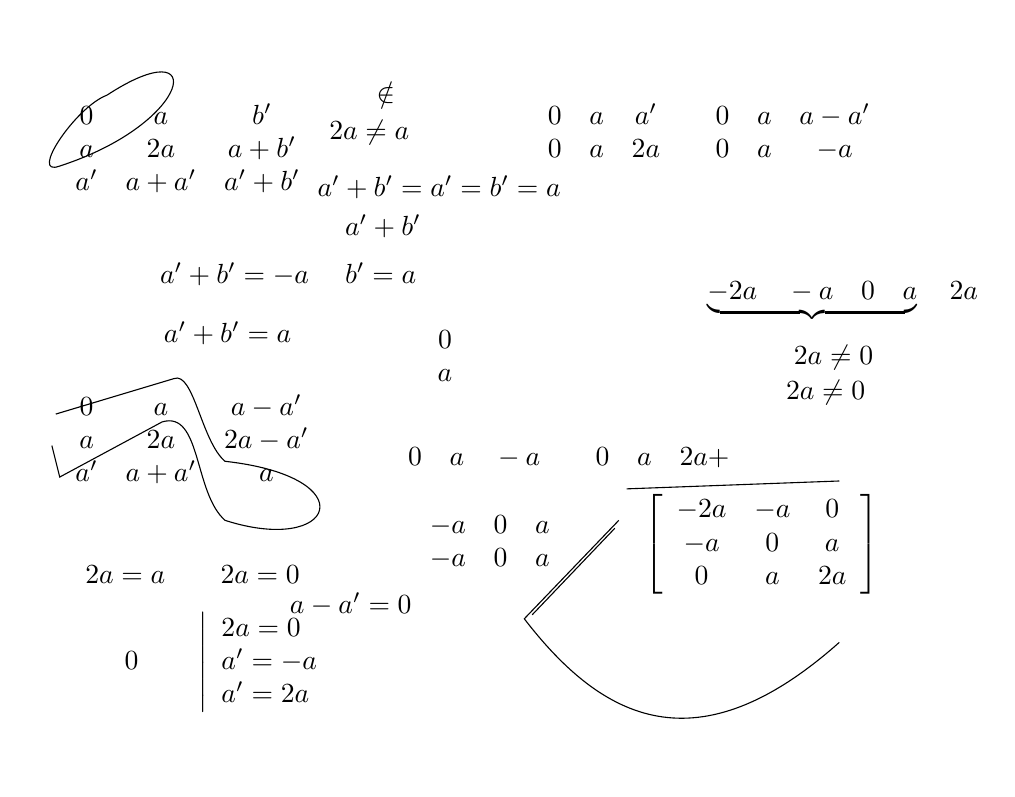
\begin{tikzpicture}[x=1cm,y=1cm]
\node[anchor=north west] at (0,0) {$\begin{array}{ccc}0&a&\deleted{b'}\\a&\deleted{2a}&\deleted{a+b'}\\\deleted{a'}&\deleted{a+a'}&a'+b'\end{array}$};
\draw (0.7,-0.05) .. controls (2.0,0.8) and (1.8,-0.4) .. (0.1,-0.95) .. controls (-0.3,-1.1) and (0.3,-0.2) .. (0.7,-0.05);
\node[anchor=north west] at (4.0,0.25) {$\deleted{\unsure{\notin}}$};
\node[anchor=north west] at (3.4,-0.25) {$\deleted{2a\ne a}$};
\node[anchor=north west] at (3.25,-0.95) {$\deleted{\unsure{a'+b'=a'=b'=a}}$};
\node[anchor=north west] at (3.6,-1.45) {$\deleted{\unsure{a'+b'}}$};
\node[anchor=north west] at (1.25,-2.05) {$\deleted{\unsure{a'+b'=-a}}$};
\node[anchor=north west] at (3.6,-2.05) {$\deleted{b'=a}$};
\node[anchor=north west] at (1.3,-2.8) {$a'+b'=a$};
\node[anchor=north west] at (4.6,-2.85) {$\begin{array}{c}0\\a\end{array}$};
\node[anchor=north west] at (6.0,0) {$\begin{array}{ccc@{\qquad}ccc}0&a&a'&0&a&\uline{a-a'}\\0&a&2a&0&a&-a\end{array}$};
\node[anchor=north west] at (8.2,-2.3) {$\underbrace{-2a\quad -a\quad0\quad a}\quad2a$};
\node[anchor=north west] at (9.3,-3.1) {$\deleted{\unsure{2a\ne0}}$};
\node[anchor=north west] at (9.2,-3.55) {$2a\ne0$};
\node[anchor=north west] at (0,-3.7) {$\begin{array}{ccc}0&a&\uline{a-a'}\\a&\uline{2a}&2a-a'\\\uline{a'}&\uline{a+a'}&a\end{array}$};
\draw (0.05,-4.1) -- (1.55,-3.65) .. controls (1.8,-3.55) and (1.9,-4.45) .. (2.2,-4.7) .. controls (4.0,-4.9) and (3.6,-5.9) .. (2.2,-5.45) .. controls (1.8,-5.1) and (1.9,-4.05) .. (1.4,-4.2) -- (0.1,-4.9) -- (0,-4.5);
\node[anchor=north west] at (0.3,-5.9) {$\deleted{\unsure{2a=a}}\qquad\deleted{2a=0}$};
\node[anchor=north west] at (2.9,-6.25) {$\deleted{\unsure{a-a'=0}}$};
\node[anchor=north west] at (0.8,-6.5) {$0\qquad\left|\begin{array}{l}2a=0\\a'=-a\\a'=2a\end{array}\right.$};
\node[anchor=north west] at (4.4,-4.4) {$\deleted{0\quad a\quad -a\qquad0\quad a\quad2a\unsure{+}}$};
\node[anchor=north west] at (4.5,-5.2) {$\begin{array}{ccc}-a&\deleted{0}&\deleted{a}\\-a&0&a\end{array}$};
\node[anchor=north west] at (7.4,-5.0) {$\left[\begin{array}{ccc}-2a&-a&0\\-a&0&a\\0&a&2a\end{array}\right]$};
\draw (7.3,-5.05) -- (10.0,-4.95);
\draw (7.2,-5.45) -- (6.0,-6.7) .. controls (7.0,-8.0) and (8.2,-8.6) .. (10.0,-7.0);
\draw (7.15,-5.55) -- (6.1,-6.65);
\end{tikzpicture}}
% archive foliation: 14
\scanpage{16}
% The manuscript is upside down in the supplied scan; reading order below follows the writing.
\deleted{``cellules'' des décompositions cellulaires ``à la Bruhat'' des espaces homogènes projectifs sous des groupes semi-simples. Le cas particulier des ``cycles de Schubert'' sur les variétés grassmanniennes permet justement de développer des conséquences d'intérêt général en topologie différentielle.}

\margin{$x^2=u$}
\[
\begin{aligned}
(V_1\dotplus\{x\})\ast(V_1\dotplus\{\unsure{x|u}\})
&=2V_1\dotplus\{u\}+2\{x\}\ast V_1\\
&=2G+\{u\}
\end{aligned}
\]
\diagram{\begin{array}{ccccc}
&&\inserted{V_1\dotplus\{x\}}&&\\
\{e\}&V_1&\deleted{\unsure{\{x\}\ast V_1}}&V_2&\\
&\multicolumn{2}{c}{\unsure{\longleftrightarrow}}&&
\end{array}}
\[
\deleted{2V_1+\unsure{u}}\qquad\boxed{3\ 2\ 2\ 2}
\]
\[
E\ast F\qquad\begin{array}{l}a+b=a'+b'\\(a-a')=(b'-b)\end{array}
\]
\[
a_1+a_2\qquad b_1+b_2
\]
\[
\deleted{a_1}\qquad a\qquad 0\ a\ \big/\ 0\ \deleted{\unsure{b+a}}\ a
\]
\[
\unsure{-}\qquad\deleted{0\quad a}\quad0\quad a,a\quad2a\qquad a\ne0
\]
\[
\deleted{2a\ne0}\qquad 2a=0
\]
\diagram{\begin{array}{cc}
\begin{array}{llll}1&1&1&1\\2&1&1&\end{array}&
\begin{array}{llll}2&2&&\\2&1&1&\\\deleted{\unsure{2|4}}&1&1&1\end{array}
\end{array}}
\figure{\begin{tikzpicture}\draw (0,0)--(0.8,1.6);\end{tikzpicture}}
\[
V_1\ast(V_1+\{x\})=2V_1+x\ast V_1
\]
\[
\uline{V_1+G}
\]
\diagram{\begin{array}{cc}
\begin{array}{llllll}2&2&1&1&&\\1&1&1&1&1&1\\2&1&1&1&&\\\deleted{\unsure{2}}&\deleted{\unsure{1}}&\deleted{\unsure{1}}&\unsure{1}&&\end{array}
&\begin{array}{ccc}E+&x\ast&E\\3&&3\\&&\deleted{\unsure{E+xE}}\end{array}
\end{array}}
% archive foliation: 15
\scanpage{17}
\[
E_i=[\unsure{-i|i},i]\qquad0\leq i\leq m
\]
\margin{NB $E_m=G$, $E_{\unsure{1|0}}=\varepsilon$}
\[
F_{\unsure{i|j}}=[m-j,m+1+j]\qquad0\leq j\leq m-1\qquad F_m=E_m=G
\]
\inserted{\[
E_i\ast E_j=\sum\alpha_{ij}^h E_h\qquad\alpha_{ij}^h\geq0
\]}
\[
F_i\ast F_j=\sum_0^m\beta_{ij}^h E_h\qquad\beta_{ij}^h\geq0
\]
\[
E_i\ast F_j=\sum\gamma_{ij}^h F_h
\]
\margin{$\varepsilon=\varepsilon^{-1}$\quad\deleted{$\unsure{\varepsilon}$}}
\[
\mathcal A(\uline{g,\deleted{\unsure{\delta}}\varepsilon})=
\left\{\begin{array}{ll}
\dfrac g2\ast\mathcal A(0)&\text{si }\varepsilon=+1\\
\dfrac g2\ast\mathcal B(0)&\text{si }\varepsilon=-1
\end{array}\right.
\]
\[
\mathcal A(\tilde g)\ast\mathcal A(\tilde h)\unsure{\subset|\subseteq}\mathcal A(\tilde g\cdot\tilde h)
\]

% The following portion is written in the opposite orientation.
\deleted{$\unsure{G'}\quad G'\text{ groupe}\quad G'\xrightarrow{\lambda}G$}
\[
\tilde G\text{ gr}\qquad\tilde G\xrightarrow{\rho}G\quad\text{hom.}
\]
\[
i:{}_2G\simeq\operatorname{Ker}\rho
\]
\margin{\deleted{\unsure{f}}\quad
$\begin{aligned}
A&=g\ast\unsure{\check A|\tilde A}=\check A\ast g\\
B&=h\ast\check B=\check B\ast h\\
A\ast B&=g\ast\check A\ast h\ast\check B=\unsure{g\ast\check A\ast\check B\ast h}
\end{aligned}$}
\[
\forall\tilde g\in G\qquad\mathcal A(\tilde g)\subset\mathcal P_f(G),
\]
\margin{On pose $C(\tilde g)$ cône des
$\displaystyle\sum_{A\in\mathcal A(\tilde g)}\alpha_A\unsure{A_\ast|A}$, $\alpha_A\geq0$}

a) $\mathcal A(\tilde g)$ \unsure{tot} ordonné

b) $A\in\mathcal A(\tilde g)\Longrightarrow A=\deleted{\unsure{\rho(\tilde g)}}g\ast\check A$ où $g=\rho(\tilde g)$
\margin{$\forall\tilde g\in\tilde G$}

c) $A\in\mathcal A(\tilde g),\ B\in\mathcal B(\tilde h)\Longrightarrow A\ast B\in C(\tilde g\tilde h)$
\margin{$\forall\tilde g,\tilde h\in\tilde G$}

d) Si $u\in{}_2G$, $\tilde g\in G$, \unsure{$\ldots$}

\deleted{d) $\mathcal A(\tilde g\tilde u^2)=\tilde u\ast\mathcal A(\tilde g)\quad\mathcal A(\unsure{\tilde u\tilde g})=$}
$\mathcal A(i(u)\tilde g)=u\ast\mathcal A(\tilde g)$

d) $\forall\tilde g,\tilde h\in\tilde G\quad\exists s\in G$ tel que $\mathcal A(\tilde g)\cup\unsure{\varepsilon_s|s}\mathcal A(\tilde h)$ tot. ordonné

[i.e. $\bigcup\mathcal A_g$
% archive foliation: 16
\scanpage{18}
\begin{center}
UNIVERSITE DES SCIENCES\\
ET TECHNIQUES\\
DU LANGUEDOC\\
\figure{\begin{tikzpicture}\draw (0,0)--(1.5,0);\end{tikzpicture}}

PROFESSEURS SANS CHAIRE ET MAITRES DE CONFERENCES

PROPOSITIONS RELATIVES A L'AVANCEMENT POUR L'ANNEE 1979
\end{center}
Service du Personnel\qquad/MV

\diagram{\begin{array}{|l|c|c|c|c|c|c|c|c|c|}
\hline
\begin{array}{l}\text{Noms et Ordre}\\\text{de présentation}\end{array} & \begin{array}{l}\text{Section}\\\text{C.C.U.}\end{array} & \begin{array}{l}\text{Date de}\\\text{naissance}\end{array} & \begin{array}{l}\text{Date d'entrée}\\\text{dans l'Enseign.}\\\text{supérieur}\end{array} & \begin{array}{l}\text{Classement}\\\text{actuel}\end{array} & \begin{array}{l}\text{Date dernière}\\\text{promotion}\\\text{d'échelon}\end{array} & \begin{array}{l}\text{Ancienneté au}\\\text{31-12-1978}\\\text{(échelon)}\end{array} & \begin{array}{l}\text{Classe}\\\text{et échelon}\\\text{proposés}\end{array} & \text{Choix} & \text{Ancienneté}\\\hline
\text{GRIMAUD J.} & \text{27°} & \text{7.10.39} & \text{1.10.62} & \text{5°éch.} & \begin{array}{l}\text{1.01.77}\\\text{(avec 2a 8m21j.}\end{array} & \text{4a 8m 21j} & \text{6°éch.} & \text{1.01.79} & \text{-}\\
\text{HEBANT Ch.} & \text{30° 4°} & \text{7.05.41} & \text{1.12.61} & \text{4°éch.} & \begin{array}{l}\text{1.10.77}\\\text{(avec 9m)}\end{array} & \text{2a} & \text{5°éch.} & \text{-} & \text{1.01.79}\\
\text{HINZELIN P.} & \text{49°} & \text{2.10.41} & \text{1.10.63} & \text{3°éch.} & \text{1.04.77} & \text{1a 9m} & \text{4°éch.} & \text{1.01.79} & \text{1.04.79}\\
\text{JOUANNA P.} & \text{49°} & \text{23.10.33} & \text{1.12.68} & \text{5°éch.} & \begin{array}{l}\text{1.01.79}\\\text{(avec 3 a)}\end{array} & \text{3a} & \text{6°éch.} & \text{1.07.79} & \text{-}\\
\text{LANCELOT J.} & \text{24°} & \text{23.08.42} & \text{1.10.77} & \text{2°éch.} & \text{1.06.78} & \text{7m} & \text{3°éch.} & \text{1.09.79} & \text{-}\\
\text{LAPASSET J.} & \text{21° 2°} & \text{17.12.37} & \text{1.11.63} & \text{5°éch.} & \begin{array}{l}\text{1.01.76}\\\text{(avec 4m 23j)}\end{array} & \text{3a 4m 23j} & \text{6°éch.} & \text{1.03.79} & \text{-}\\
\text{LAPSCHER F.-} & \text{18° 2°} & \text{29.03.35} & \text{1.06.64} & \text{5°éch.} & \text{1.02.75} & \text{3a 11m} & \text{6°éch.} & \text{1.01.79} & \text{-}\\
\text{LEBLEU B.} & \text{29°} & \text{8.03.45} & \text{1.10.77} & \text{1°éch.} & \text{1.10.77} & \text{1a 3m} & \text{2°éch.} & \text{1.01.79} & \text{1.10.79}\\
\text{LIEGEOIS A.} & \text{23°} & \text{27.12.40} & \text{1.10.74} & \text{3°éch.} & \text{1.01.78} & \text{1a} & \text{4°éch.} & \text{1.04.79} & \text{-}\\
\text{LOUIS P.} & \text{24°} & \text{28.06.31} & \text{1.07.59} & \text{5°éch.} & \begin{array}{l}\text{1.01.74}\\\text{(avec 3m)}\end{array} & \text{5a 3m} & \text{6°éch.} & \text{1.01.79} & \text{1.10.79}\\
\text{MACHEIX J.J.} & \text{30° 4°} & \text{2.04.39} & \text{1.10.60} & \text{4°éch.} & \text{1.01.78} & \text{1a} & \text{5°éch.} & \text{1.04.79} & \text{-}\\
\text{MATHIEU H.} & \text{21°} & \text{19.04.40} & \text{1.10.63} & \text{5°éch.} & \begin{array}{l}\text{1.01.79}\\\text{(avec 4a 1m)}\end{array} & \text{4a 1m} & \text{6°éch.} & \text{1.01.79} & \text{-}\\
\text{NOUGIER J.P.} & \text{23°} & \text{5.07.39} & \text{1.11.64} & \text{5°éch.} & \text{1.04.76} & \text{2a 9m} & \text{6°éch.} & \text{1.10.79} & \text{-}\\
\text{RIBES M.} & \text{27°} & \text{15.05.41} & \text{1.10.64} & \text{3°éch.} & \begin{array}{l}\text{1.10.78}\\\text{(avec 1a)}\end{array} & \text{1a 3m} & \text{4°éch.} & \text{1.01.79} & \text{1.10.79}\\
\text{SANS A.} & \text{31° 1°} & \text{14.12.39} & \text{1.10.60} & \text{4°éch.} & \text{1.04.77} & \text{1a 9m} & \text{5°éch.} & \text{1.01.79} & \text{1.04.79}\\
\begin{array}{l}\text{TARODO DE LA}\\\text{FUENTE B.}\end{array} & \text{50°} & \text{22.07.37} & \text{1.10.61} & \text{4°éch.} & \text{1.01.77} & \text{2a} & \text{5°éch.} & \text{-} & \text{1.01.79}\\
\text{VITSE P.} & \text{27° 2°} & \text{1.10.39} & \text{1.11.63} & \text{5°éch.} & \begin{array}{l}\text{1.01.77}\\\text{(avec 9m 6j)}\end{array} & \text{2a 9m 6j} & \text{6°éch.} & \text{1.10.79} & \text{-}\\
\hline
\end{array}}
% archive foliation: 17
\scanpage{19}
\textcircled{1}\quad $|f,g|$

\deleted{\unsure{Soit}} $G$ un ensemble, $C(G)=\mathbb R[G]=\mathbb R^{(G)}$, (fonctions réelles à support fini), $\mathbb R[G]^+=\{f\in\mathbb R[G]\mid f\geq0\}$

\deleted{$\unsure{f,g\in}$} Eparpillement $f'$ de $f$ (ou $f,f'$ équivalentes, on écrit $f'\sim f$) sss $\exists\sigma\in\unsure{\mathfrak S_G},\ f'=f\circ\sigma$ $\Longleftrightarrow$ la suite des valeurs $\ne0$ de $f$, \deleted{\unsure{comptées}} rangées en décroissant et avec multiplicités, sont les \deleted{\unsure{mêmes}} $\Longleftrightarrow f(\mu)=f'(\mu)$ (image directe de la mesure canonique).
\margin{Notation $A(f)$, condition $A(f')=A(f)$}

Si $f,g\in\mathbb R[G]^+$, on pose
\[
|f,g|=\operatorname{Sup}_{f'\sim f}\langle f',g\rangle
=\operatorname{Sup}_{g'\sim g}\langle f,g'\rangle
=\operatorname{Sup}_{\substack{f'\sim f\\g'\sim g}}\langle f',g'\rangle
\]
\margin{\uline{NB} $|f,g|=|f',g'|$ si $f'\sim f$, $g'\sim g$}

\deleted{\uline{Proposi}} Pour que $\langle f',g'\rangle$ réalise le Sup, il f. et s. que pour $\forall\alpha,\beta\in\mathbb R^{+\ast}$, $E_\alpha(f')$ et $E_\beta(g')$ soient en relation d'inclusion (i.e. $\subset$ ou $\supset$), i.e. il f. et s. que $E_\ast(f')\cup E_\ast(g')$ soit \unsure{tot} ordonné $\Longleftrightarrow\exists$ un ordre total sur $G$ [si $G$ est fini ou dénombrable] $\sim[0,n]$ ou $\mathbb N$, tel que $f$ et $g$ soient \unsure{décroissantes}.

\uline{NB} On pose $E_\alpha(f)=\{s\in G\mid f(s)\geq\alpha\}$ (donc $\alpha\leq\beta\Rightarrow E_\alpha(f)\supset E_\beta(f)$) et $E_\ast(f)=\{E_\alpha(f)$

\margin{\uline{NB} Si $f\sim g$ alors le Sup est réalisé ssi $f'=g'$ et
$|f,g|=|f,f|=|g,g|=\|f\|_2^2=\displaystyle\int_G f^2$}

\uline{Propositi} $f'\sim f\Longleftrightarrow\forall g\in C(G)^+,\ |f',g|=|f,g|\Longleftrightarrow\forall A\in\mathcal P_f(G),\ |f',A|=|f,A|$

\textcircled{2}\quad \uline{$f'\prec f$}

\uline{Prop.} Conditions équivalentes sur $f',f\in\mathbb R[G]^+$

a) $\forall g\in\unsure{\mathbb R(G)^+|\mathbb R[G]^+}$, on a
\[
|f',g|\leq|f,g|
\]
b) $\forall A\in\mathcal P_f(G)$, \unsure{$\ldots$}
\[
|f',A|\leq|f,A|
\]
c) \deleted{\unsure{$\forall$}} $\unsure{n|p}\in\mathbb N^{\unsure{\ast|0}}$, on a
\[
\sum_0^{\unsure{n|m}}A(f')_i\leq\sum_0^{\unsure{n|m}}A(f)_i.
\]
\margin{On écrit alors $f'\prec f$}
% archive foliation: 18
\scanpage{20}
\uline{NB} C'est une relation \deleted{d'ordre} \inserted{de préordre}. La relation d'équ. associée est $f'\sim f$.
\margin{\uline{NB} Le sup de $\langle f',g\rangle$ pour $f'\prec f$ est atteint \deleted{pour} \inserted{des} $f'\sim f\ldots$}

\deleted{\uline{Cor} $f'\prec f$, $g'\prec g\Longrightarrow|f',g'|\leq|f,g|$}

\uline{Cor} $f'\prec f\Longleftrightarrow\forall g',g\in C(G)^+$, avec $g'\prec g$, on a
\[
|f',g'|\leq|f,g|
\]

\uline{3}\quad\uline{Couples \unsure{pritorisés|priorisés}}

A partir de maintenant, $G$ est un groupe, d'où opération $f\ast g$ sur $\mathbb R[G]^{\unsure{\ast|+}}$, $\mathbb R[G]^+$ est stable.

\margin{\uline{NB} Soient $f,g\in\mathbb R(G)^+$. Considérons les $\|f'\ast g\|_\infty$ ou $(f'\ast g)(0)$ pour $f'\prec f$, alors le Sup est \deleted{\unsure{atteint}\ $\unsure{\|f\ast g\|_\infty}$} \inserted{$=$}, et il est atteint pour $f'\sim f$.}

\uline{Prop} $f,g\in\mathbb R(G)^+$, Conditions équivalentes

a) $f'\prec f$, $g'\prec g$, $\|f'\ast g'\|_\infty\leq\|f\ast g\|_\infty$

b) $\forall f'\prec f$, $g'\prec g$
\[
\underset{\inserted{=\langle f',\check g'\rangle}}{(f'\ast g')(0)}
\leq\operatorname{Sup}_{s\in G}
\underbrace{(f\ast g)(s)}_{\inserted{=\deleted{\unsure{\langle f,\check g\rangle}}\langle f\unsure{\ast|,}\varepsilon_s\check g\rangle}}
\]
a') \deleted{$\unsure{\forall f'\sim f,\ \forall g'\sim g}$} a), b) avec $f'\sim f$, $g'\sim g$

c) $|f,g|=\|f\ast g\|_\infty$

d) $\exists s\in G$ tel que
\diagram{\begin{tikzcd}[row sep=small]
\inserted{E_\ast(g)\cup E_\ast(\check f\ast\varepsilon_s)\ \deleted{\unsure{E_\ast(\check g)}}\ \text{tot. ordonné}}\arrow[d,leftrightarrow]\\
E_\ast(f)\cup E_\ast(\varepsilon_s\check g)\quad\text{tot. ordonné}
\end{tikzcd}}
i.e. $\forall\alpha,\beta\in\mathbb R^{+\ast}$, $E_\alpha(f)$ et $E_\beta(\varepsilon_s\check g)$ en relation d'inclusion

\uline{Def} On dit alors que le \deleted{\unsure{bi}}couple $(f,g)$ est \uline{\unsure{pritorisé|priorisé}}
([Il n'est pas clair que la relation soit symétrique --- \deleted{\unsure{elle signifie}\ $\forall s$} mais OK si $G$ commutatif])

\uline{Cor} $f\in\mathbb R[G]^+$, \deleted{\unsure{alors}} $(f,f)$ est \unsure{pritorisé|priorisé} (\deleted{\unsure{sss}\ $f\text{ et }f$} \inserted{$\exists s\in G$} tel que $\check f=\varepsilon_s\ast f$ ($\Longleftrightarrow\check f=f\ast\varepsilon_s$)

\margin{\figure{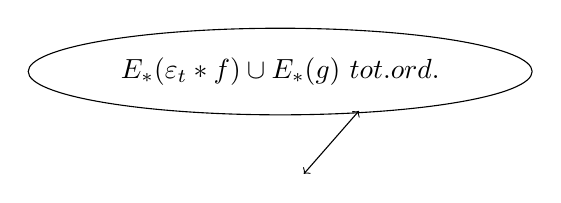
\begin{tikzpicture}[x=1cm,y=1cm]
\node at (0,0) {$E_\ast(\varepsilon_t\ast f)\cup E_\ast(g)\ \text{tot. ord.}$};
\draw (0,0) ellipse (3.2cm and .55cm);
\draw[<->] (1,-.5) -- (.3,-1.3);
\end{tikzpicture}}}
\uline{NB} Si dans la prop. $g$ satisfait la condition précédente, alors la condition de la prop signifie aussi \unsure{eq} $\exists t\in G$ t.q. $E_\ast(f)\cup E_\ast(\varepsilon_t\ast g)$ tot. ordonné
% archive foliation: 19
\scanpage{21}
\deleted{\unsure{4}}
Donc si $f$ et $g$ sont sym. à translation près, la condition $(f,g)$ \unsure{pritorisé|priorisé} est une condition \uline{symétrique} en $f,g$.

4. \uline{Couples bons.}
\[
f,g\in\mathbb R[G]^+.
\]
\margin{Cette condition est inv. par translation. \deleted{\unsure{Donc}} Si $(f,g)$ est bon, $\check g,\check f$ aussi. Donc si $f,g$ sont sym. mod translation, alors $(f,g)$ bon sss $(g,f)$ bon.}

\uline{Prop} Conditions équivalentes

a) $f'\prec f$, $g'\prec g\Longrightarrow f'\ast g'\prec f\ast g$

b) $f'\sim f$, $g'\sim g\Longrightarrow f'\ast g'\prec f\ast g$

c) $\forall h\in\mathbb R[G]^+$
\[
\operatorname{Sup}_{\substack{f'\prec f\\g'\prec g\\h'\prec h}}
(f'\ast g'\ast h')(0)
\leq\operatorname{Sup}_{\substack{\deleted{\unsure{h'\prec h}}\\h'\sim h}}f\ast g\ast h'(0)
\]
\[
\begin{gathered}\Vert\\\left(\operatorname{Sup}_{h'\sim h}\|f\ast g\ast h'\|_\infty\right.\end{gathered}
\]
c') $\forall A\in\mathcal P_f(G)$,
\[
\operatorname{Sup}_{\substack{A'\sim A\\f'\sim f\\g'\sim g}}f'\ast g'\ast A'(0)
\leq\operatorname{Sup}_{A'\sim A}f\ast g\ast A'(0)
\]
\[
\begin{gathered}\Vert\\\left(\operatorname{Sup}_{A'\sim A}\|f\ast g\ast A'\|_\infty\right.\end{gathered}
\]
Cela implique que $(f,g)$ est \uline{\unsure{pritorisé|priorisé}}

\uline{Cor} Soit $S\subset\mathbb R[G]^+$, $S$ \uline{stable par $\ast$}.
\deleted{Pour que}\inserted{Conditions équiv. :}

\deleted{$S$ soit} a) $\unsure{\forall|\text{tt.}}$ couples $(f,g)\in S\times S$ sont bons, \deleted{il f. et s.}

b) \deleted{que} pour \deleted{tout} $n\in\mathbb N$, $n\geq2$, $f_1,\ldots,f_n\in S$, $f'_1,\ldots,f'_n\in\mathbb R(G)^+$
$f'_1\prec f_1\ldots$, $f'_n\prec f_n$ implique
\[
f'_1\ast\cdots\ast f'_n\prec f_1\ast\cdots\ast f_n
\]
c) [Si $\forall n\in\mathbb N^\ast$, \inserted{$n\leq\operatorname{card}G$}, $(\exists A\in S\cap\mathcal P_f(G)$ tel que $\operatorname{card}A=n$]
\margin{$\longrightarrow$ ``Condition $K$''}
\margin{condition $K$ $\Updownarrow$ \unsure{hyp}}
\[
f'_1\prec f_1,\ldots,f'_n\prec f_n\quad(f'_i\in\mathbb R(G)^+,\ f_i\in S)\Longrightarrow
\]
\[
\|f'_1\ast\cdots\ast f'_n\|_\infty\leq\|f_1\ast\cdots\ast f_n\|_\infty
\]
(ou $f'_1\ast\cdots\ast f'_n(0)$

\deleted{``condition $K$'' d) $\unsure{f'_1\sim f_1,\ f'_2\sim f_2,\ \ldots}\quad f'\sim f,\ g'\sim g,\ A'\sim A\in\mathcal P_f(G)\cap S\Longrightarrow f'\ast g'\ast A'(0)\leq\|f\ast g\ast A\|_\infty$}
% archive foliation: 20
\scanpage{22}
\margin{Si $(K)$ et si les couples $\in S\times S$ sont \unsure{pritorisés|priorisés} $\updownarrow$ id}

d) $\forall A,B\in\mathcal P_f(G)\cap S$, $A'\sim A$, $B'\sim B$, \unsure{$\ldots$}
\[
A'\ast B'\prec A\ast B\qquad\text{i.e.}\quad\uline{(A,B)\text{ bon}}
\]
e) $\forall A,B,C\in\mathcal P_f(G)\cap S$, $A'\sim A$, $B'\sim B$, $C'\sim C$, \unsure{$\ldots$}
\[
\|A'\ast B'\ast C'\|_\infty\leq\|A\ast B\ast C\|_\infty
\]

\deleted{Supposons}

Quitte à \unsure{saturer} $S$, \unsure{on s.} $S$ stable par translation
\[
S_0=S\cap\mathcal P_f(G)\qquad\unsure{\text{NB}}\quad S_0\ne\varnothing
\]
Soit $f\in S$. Alors

a) $\exists t\in G\quad f=\varepsilon_t\ast\unsure{f|\check f}$
\margin{[$(f,f)$ \deleted{bon}\inserted{\uline{pri}}]}

b) les $E_\alpha(f)\in S_0$
\margin{[$(f,A)$ \deleted{bon}\inserted{\uline{pri}} pour $A\in S_0$]}

\deleted{\unsure{Donc} Soit $f\in\mathbb R[G]^+$}

Soit \deleted{$f$} $\tilde S=\{f\in\mathbb R(G)^+\mid\text{satisfait a), b)}\}$

\deleted{$\unsure{f\in S}$} i.e.
\[
\left\{\begin{array}{l}
f=\displaystyle\sum_I\alpha_i A_i\qquad\alpha_i>0\qquad A_i\in S_0\quad(A_i)\text{ tot ord.}\\
\deleted{\unsure{f}}\ \exists\unsure{s|t}\in G,\quad A_i=\deleted{\unsure{\check A_i}}\varepsilon_s\ast\check A_i\quad\forall i
\end{array}\right.
\]
Soit de même
\[
\left|\begin{array}{l}
g=\displaystyle\sum_J\beta_j B_j\qquad\beta_j>0,\quad B_j\in S_0\quad(B_j)\text{ tot ord.}\\
t\in G,\qquad B_j=\varepsilon_t\ast\check B_j
\end{array}\right.
\]
On a
\[
f\ast g=\sum_{(i,j)\in I\times J}\alpha_i\beta_j A_i\ast B_j
\]

\deleted{Supposons que $\exists(C_{\unsure{n|\alpha}})$}

On a $A_i\ast B_j\in S$, donc
\[
E_\ast(A_i\ast B_j)\subset S_0
\]
\uuline{Supposons}
\[
\bigcup E_\ast(A_i\ast B_j)\quad\uline{\text{tot}}\text{ ordonné}
\]
\unsure{on veut}
\[
\bigcap_{C\in\bigcup_{ij}E_\ast(A_i\ast B_j)}C\ne\varnothing
\]
\diagram{\begin{tikzcd}
0\arrow[r]&{}_2G\arrow[r]&G\arrow[r,"2"]&G
\end{tikzcd}}
% archive foliation: 21
\scanpage{24}
\uline{Jeux de position}

a) $C$ ensemble des ``\uline{configurations}'' ou ``\uline{positions}''

b) $R\subset C\times C$, interprété comme $x\longmapsto R(x)$
\margin{$C\longrightarrow\mathcal P(C)$}
\[
\text{d'où}\qquad C_0=\{x\in C\mid R(x)=\varnothing\}\subset C
\]
\margin{(conf. \uline{terminales})}

c) $J$ ensemble des ``\uline{joueurs}''

d) $C\setminus C_0\xrightarrow{\alpha}J$ On dit que (si $x\in C\setminus C_0$) $j=\alpha(x)$ est le joueur qui a \uline{l'initiative} dans la position $x$.
\inserted{\[
C(j)=\{x\in C\setminus C_0\mid\alpha(x)=j\}\qquad
\bar C(j)=(C\setminus C_0)\setminus C(j)
\]}

e) $J\longrightarrow\mathcal P(C_0)\qquad j\longmapsto G_0(j)$ (ens. des \uline{positions terminales gagnantes pour $j$})

\uline{Partie}\quad $(x_0,x_1,\ldots,x_n,\ldots)$ suite finie ou infinie de positions, telle que pour deux termes consécutifs $x_i,x_{i+1}$, on ait
\[
x_{i+1}\in R(x_i)
\]
\margin{ne dépend que de $C,R$}

\uline{Prolongement} des parties --- parties non prolongeables ou ``\uline{terminées}'' : ce sont les parties qui sont soit infinies, soit finies, avec \deleted{\unsure{une}} \inserted{la} position finale $x_n\in C_0$.
\margin{Composition des parties (\unsure{Associativité|Associatif} --- on a une ``catégorie des positions''\ldots)}

\uline{Partie gagnée pour $j$} : partie finie (non prolongeable) dont la position finale $x_n$ est $\in G_0(j)$.
\margin{ne dépend que de $C,R$ et $G_0(j)\subset C_0$}
\margin{\uline{NB} \deleted{Si} $XY$ est gagnée pour $j$, \deleted{\unsure{donc}} $\Longleftrightarrow Y$ est gagnée pour $j$.}

\uline{Stratégie $\Sigma$/pour $j$} (ou $j$-Stratégie) : Application
\[
\Sigma:C(j)\longrightarrow\mathcal P(C)
\]
telle que $\forall x\in C(j)$, on ait
% archive foliation: 23
\scanpage{25}
\[
\Sigma(x)\subset R(x),\qquad\Sigma(x)\ne\varnothing.
\]
Cette notion ne dépend que de $C,R,C(j)\subset C\setminus C_0$.

\inserted{\uline{NB} On pose $\Sigma(x)=R(x)$ si $x\in\bar C(j)$. Donc on peut interpréter $\Sigma$ comme une application $C\setminus C_0\longrightarrow\mathcal P^*(C)$, $\Sigma(x)\subset R(x)$ et $\Sigma(x)\ne\varnothing$ $\forall x\in C\setminus C_0$, et $\Sigma(x)=R(x)$ si $x\in\bar C(j)$.}
\deleted{\uline{Stratégie \unsure{pour $j$} gagnante pour $x_0\in C$}}

Partie jouée en accord avec une Stratégie $\Sigma$ (ou \uline{compatible} avec $\Sigma$, ou $\Sigma$-partie) : cette notion est stable par composition. (On prend une sous-catégorie ayant mêmes objets, mais a priori moins de flèches)

\inserted{\uline{Lemme} Soit \deleted{\unsure{une stratégie}} $J'\subset J$, $\forall j\in J'$ soit $\Sigma_j$ une $j$-stratégie. Soit $x_0\in C$. Alors $\exists$ partie maximale d'origine $x_0$, comp. avec les $\Sigma_j$ $(j\in J')$.}

Stratégie $\Sigma$ (pour $j$) \uline{gagnante} pour $x_0\in C$ (ou \uline{position} $x_0$ \uline{gagnante} pour une Stratégie $\Sigma$) : toute partie maximale commençant en $x_0$, et jouée suivant $\Sigma$, est gagnée par $j$ (i.e. est finie, et son extrémité $x_n\in C_0$ est $\in G_0(j)$).
\margin{ne dépend que de $C,R,C(j),G_0(j)$}

\uline{Position \inserted{$x_0\in C$} gagnante pour} $j$ : telle qu'il existe une $j$-Stratégie qui soit gagnante pour $x_0$. Soit
\[
G(j)
\]
l'ens de ces positions. On a
\[
G(j)\cap C_0=G_0(j).
\]

[\uline{Proposition} Soit $J'\subset J$. Si $\bigcap_{j\in J'}G(j)\ne\varnothing$, alors $\bigcap_{j\in\unsure{J|J'}}G_0(j)\ne\varnothing$. En d'autres termes, si $\bigcap_{j\in J'}G_0(j)=\varnothing$, alors $\bigcap_{j\in J'}G(j)=\varnothing$ i.e. un $x_0\in C$ ne peut être gagnant pour tous les $j\in J'$.

Immédiat par le lemme.]
% archive foliation: 24
\scanpage{26}
\uline{Proposition}\quad \unsure{Soient|Soit} $\Sigma$ une $j$-Stratégie, $x_0\in C$ \deleted{position} gagnante pour $\Sigma$, $X=(x_0,x_1,\ldots,x_n\ldots)$ une partie (d'origine $x_0$) jouée suivant $\Sigma$, alors toutes les positions $x_i$ sont gagnantes pour $\Sigma$.

Soit en effet $Y=(y_0=x_i,y_1,\ldots,y_m,\ldots)$ une partie \inserted{maximale} jouée suivant $\Sigma$, \deleted{\unsure{et}} alors $XY$ est jouée suivant $\Sigma$ et est d'origine $x_0$ gagnante pour $\Sigma$, donc \deleted{est gagnée par $j$ donc $Y$ est finie} donc $Y$ est gagnée par $j$.

\uline{Th} On a \deleted{\unsure{rappel}}
\[
\begin{aligned}
a)\quad&G(j)\cap C(j)=\{x_0\in C(j)\mid R(x_0)\cap G(j)\ne\varnothing\}\\
b)\quad&G(j)\cap\bar C(j)=\{x_0\in\bar C(j)\mid R(x_0)\subset G(j)\}
\end{aligned}
\]
[et pour mémoire
\[
G(j)\cap C_0=\unsure{C_0|G_0}(j)
\]
].

\uline{Dém}\quad a) On suppose $x_0\in C(j)$.

\deleted{a)} 1) $\subset$ Soit $x_0\in G(j)\deleted{\cap C(j)}$, \inserted{soit} $\Sigma$ une stratégie pour $j$ gagnante pour $x_0$, considérons $x_1\in\Sigma(x_0)$, alors $(x_0,x_1)$ est une $\Sigma$-partie, donc par la prop. précédente, $x_1$ est gagnant pour $\Sigma$, donc $j$-gagnant, donc $x_1\in R(x)\cap G(j)$, donc $R(x)\cap G(j)\ne\varnothing$.

2) $\supset$ Soit $x_1\in R(x)\cap G(j)$. Prouvons que $x_0\in G(j)$. \deleted{\unsure{On défi|On déf}} Soit $\Sigma_1$ une $j$-stratégie $x_1$-gagnante. Si $x_0$ est gagnant pour $\Sigma_1$, on a $x_0\in G(j)$, OK. Sinon, définissons une $j$-stratégie $\Sigma_0$ $x_0$-gagnante ainsi :
\[
\begin{aligned}
\Sigma_0(x_0)&=\{x_1\}\\
\Sigma_0(x)&=\Sigma_1(x)\quad\text{si }x\ne x_0
\end{aligned}
\]
% archive foliation: 25
\scanpage{27}
C'est une $j$-stratégie, \deleted{prouvons} \inserted{Prouvons} qu'elle est gagnante pour $x_0$. \deleted{\unsure{ou}} Une partie maximale jouée suivant $\Sigma_0$ \unsure{commence} avec $(x_0,x_1)$, soit $(x_0,x_1,\ldots,x_m,\ldots)$ \deleted{les $x_i$ $(i\geq1)$ sont \unsure{gagnants} pour $\Sigma_1$}, prouvons qu'elle est gagnée par $j$. Prouvons que tous les $x_i$ $(i\geq1)$ sont $\ne x_0$. Sinon, \deleted{si $i$ est le} plus petit indice $i\geq1$ tel que $x_i=x_0$, \deleted{pour un $\unsure{i>1|j>1}$}, alors \deleted{par la prop. \unsure{il s'ensuivrait}} \inserted{$(x_1,\ldots,x_i=x_0)$ serait compatible avec $(\Sigma_1)$,} on aurait que $x_i\inserted{{}=x_0}$ est gagnant pour $\Sigma_1$, contrairement à la supposition que $x_0$ non gagnant pour $\Sigma_1$.

Comme les $x_i$ $(i\geq1)$ sont $\ne x_0$, la partie $(x_1,x_2,\deleted{\unsure{x_0}}\inserted{\ldots})$ est une $\Sigma_1$-partie, donc elle est gagnante pour $j$, donc $(x_0,x_1,\ldots)$ aussi; cqfd.

b) On suppose $x_0\in\bar C(j)$.

1) $\subset$. Supposons $x_0\in G(j)$, prouvons $R(x)\subset G(j)$, Soit $x_1\in R(x)$, prouvons $x_1\in G(j)$. En effet, \inserted{si $\Sigma_0$ est une $j$-stratégie $x_0$-gagn.}, $(x_0,x_1)$ est une \inserted{$\Sigma_0$-}partie, donc par la prop., $x_1$ est gagnant pour $\Sigma_0$, donc $x_1\in G(j)$.

2) $\supset$. Supposons $R(x_0)\subset G(j)$, prouvons $x_0\in G(j)$. $\forall x_1\in R(x_0)$, soit $\Sigma_{x_1}$ une $j$-stratégie $x_1$-gagnante. Choisissons un \uline{bon ordre} sur $R(x_0)$. On va définir une $j$-stratégie $\Sigma_0$ $x_0$-gagnante ainsi :

$\forall x\in C$, soit
\[
E(x)=\{x_1\in R(x_0)\mid\exists\ \Sigma_{x_1}\text{-partie de }\unsure{x_0|x_1}\text{ à }x\}
\]
% archive foliation: 26
\scanpage{28}
Soit
\[
C'=\{x\in C\mid E(x)\ne\varnothing\}
\]
et pour $x\in C'$, posons
\[
\varepsilon(x)=\text{plus petit élément de }E(x)
\]
(donc $\varepsilon:C'\longrightarrow R(x_0)$). Posons
\[
\Sigma_0(x)=\begin{cases}
R(x)&\text{si }\deleted{\unsure{\forall}}x\in\bar C(j)\cup\complement C'\\
\Sigma_{\varepsilon(x)}(x)&\text{si }x\in C(j)\cap C'
\end{cases}
\]
Donc $\Sigma_0$ est une $j$-Stratégie. On va prouver qu'elle est gagnante pour $x_0$.

\uline{Lemme}\quad \deleted{On a} \inserted{Si $x\in C'$, $x$ est gagnant pour $\Sigma_{\varepsilon(x)}$ (donc gagnant pour $j$ --- donc $C'\subset G(j)$) et} \deleted{$C'\subset G(j)$, et si $x\in C'$, $y\in\Sigma_0(x)$,} alors \deleted{$\Sigma_0(x)\subset C'$ et} pour $\unsure{\forall|\text{tt.}}\,y\in\Sigma_0(x)$, on a
\[
E(y)\ni\unsure{E(x)|\varepsilon(x)}
\]
(donc $E(y)\ne\varnothing$ donc $y\in C'$, donc $\Sigma_0(x)\subset C'\inserted{\subset G(j)}$) et par suite
\[
\varepsilon(y)\leq\varepsilon(x).
\]

\uline{Dém}\deleted{\unsure{cq}}
Soit $x\in C'$ donc $E(x)\ne\varnothing$, alors si $x_1\in E(x)$ $\exists$ \deleted{partie} $\Sigma_{x_1}$-partie de $x_1$ à $x$, donc par la prop. (comme $\Sigma_{x_1}$ est $x_1$-gagnante), $x$ est $\Sigma_{x_1}$-gagnante, donc à fortiori $x\in G(j)$.

Soit $y\in\Sigma_0(x)=\Sigma_{\varepsilon(x)}(x)$
\[
(\underset{\substack{\Vert\\\varepsilon(x)}}{x_1},x_2,\ldots,x_m=x,x_{\unsure{m+1|m-1}}=y)
\]
est une $\Sigma_{\varepsilon(x)}$-partie, donc \deleted{$\unsure{\varepsilon_0}$} $\varepsilon(x)\in E(y)$, OK.

Prouvons que $\Sigma_0$ est gagnante pour $x_0$.
Soit une partie maximale commençant par $x_0$
% archive foliation: 27
\scanpage{29}
et comp. avec $\Sigma_0$
\[
(x_0,x_1,x_2,\ldots)
\]
Par le lemme, on voit de proche en proche \deleted{cette partie est} \inserted{(puisque $x_1\in C'$)} que \deleted{$x_1\in G(j)$, $x$} les $x_i$ $(i\geq1)$ sont $\in C'\deleted{\cap G(j)}$ donc $j$-gagnants. Pour montrer que la partie est gagnée par $j$, il suffit de prouver qu'elle est finie. \deleted{Or} \inserted{Supposons le contraire.} Les $\varepsilon(x_i)$ $(i\geq1)$ forment une suite décroissante d'éléments de $R(x_0)$, donc stationnaire. Soit $n$ tel que $\varepsilon(x_m)=\varepsilon(x_n)\inserted{(=\unsure{\xi|\zeta})}$ pour $m\geq n$.

Alors par définition de $\Sigma_0$, la partie $(x_n,x_{n+1},\ldots,\ )$ est une partie comp. avec $\Sigma_{\unsure{\xi|\zeta}}$. Comme $x_n$ est gagnant pour $\Sigma_{\unsure{\xi|\zeta}}$ (par le lemme), cette partie est finie, absurde.

Stratégie \uline{contre $j$} (\unsure{stratégie relative à} $\bar C(j)$, i.e. $\Sigma'$ telle que $\Sigma'(x)=R(x)$ si $x\in C(j)$ (et $\Sigma'(x)\subset R(x)$, $\Sigma'(x)\ne\varnothing$ si $x\in\bar C(j)$) admissible pour $x_0$ (tte partie maximale d'origine $x_0$ jouée suivant $\unsure{x_0|\Sigma'}$ est \uline{non gagnée} par $j$, i.e. est ou bien infinie, ou bien a une position terminale $\notin\unsure{C_0|G_0}(j)$).

\deleted{\uline{Corollaire}} \inserted{Théorème} Soit $\Sigma'$ la stratégie contre $j$ définie par
% archive foliation: 28
\scanpage{30}
\[
\Sigma'(x)=\begin{cases}
R(x)&\text{si }x\in C(j)\cup G(j)\\
R(x)\cap\complement G(j)&\text{si }x\in\bar C(j)\cap\complement G(j)
\end{cases}
\]
(C'est une stratégie contre $j$, par [b) $\supset$]. Alors Pour $x\in C$, les conditions suivantes sont équivalentes

a) $x_0\notin G(j)$

b) $x_0$ est admissible contre $j$

c) $x_0$ est admissible pour $\Sigma'$ contre $j$.

\uline{Dém}\quad c) $\Longrightarrow$ b) trivial, b) $\Longrightarrow$ a) par le lemme, Prouvons a) $\Longrightarrow$ c). \unsure{Si on a} une partie $(x_0,x_1,\ldots)$ d'origine $x_0$ jouée en accord avec $\Sigma'$, alors par définition de $\Sigma$, on voit de proche en proche que $x_i\in\complement G(j)$ $\forall i$, donc la partie ne peut être gagnée par $j$ !

\uline{Corollaire}\quad Supposons $J=\{j,j'\}$, $j\ne j'$, et
\margin{$\big|$}
\[
G_0(j)\cap G_0(j')=\varnothing.
\]
Soit \deleted{$\unsure{N}$}
\[
N=\{x\in C\mid x\text{ admissible contre }j,\text{ et contre }j'\}.
\]
\margin{$\big|$}
Alors $C$ est réunion disjointe de $G(j)$, $G(j')$ et $N$.
% archive foliation: 29
\scanpage{31}
\deleted{Supposons}
\uline{NB}\quad $G(j),G(j')$ et $N(j)$ sont connus quand on connaît (en plus des \inserted{parties} $G_0(j)$ et $G_0(j')$ de $C_0$) les ensembles
\[
\left\{\begin{aligned}
G^*&=\{x\in C\setminus C_0\mid x\in G(\alpha(x))\}\\
P^*&=\{x\in C\setminus C_0\mid x\in G(\bar\alpha(x))\}
\end{aligned}\right.
\]
où $\bar\alpha(x)$ désigne l'unique $j'\in J$ tel que $j'\ne j=\alpha(x)$.

On dit qu'une position $x\in C\setminus C_0$ qui est $\in G^*\inserted{\text{ (resp. }\in P^*\text{)}}$, i.e. \deleted{telle} \inserted{gagnante} \unsure{pour} le joueur qui a l'\unsure{initiation|initiative} (resp. pour le joueur qui n'a pas l'initiative) est \uline{gagnante} (resp. \uline{perdante}); on dit que c'est une \uline{position nulle} \deleted{autrement} si elle n'est ni gagnante, ni perdante, on pose
\[
N^*=(C\setminus C_0)\setminus(G^*\cup P^*)=N\cap(C\setminus C_0)
\]
(où $N$ est défini dans le corollaire ci-dessus).

On aura
\[
\left\{\begin{aligned}
G(j)\cap C(j)&=G^*\cap C(j)\\
G(j)\cap\bar C(j)&=G(j)\cap C(j')=P^*\cap C(j')\\
G(j)\cap C_0&=G_0(j)
\end{aligned}\right.
\]
ce qui montre que \inserted{les} $G(j)$ $(j\in\unsure{G|J})$ se reconstituent par la connaissance de $G^*,P^*$ et des $G_0(j)$ $(j\in J)$.

Supposons qu'on ait une application
\[
\hat\alpha:C\longrightarrow J
\]
prolongeant $\alpha$, et qu'on ait, pour $\forall x\in C$ et $y\in R(x)$
\[
\hat\alpha(y)\ne\hat\alpha(x)
\]
% archive foliation: 30
\scanpage{32}
On dit alors que le jeu \unsure{est|de} position à deux joueurs est un jeu \uline{alterné} (les deux joueurs jouent alternativement). Pour qu'une application $\hat\alpha$ existe prolongeant $\alpha$ et ayant les propriétés précédentes, il f. et s. que les \unsure{deux} conditions suivantes soient satisfaites

1) $\forall x,y\in C$, tels que $y\in R(x)$, $y\notin\deleted{\unsure{G_0|C_0}} C_0$, on a $\alpha(y)\ne\alpha(x)$

2) $\forall y\in C_0$, soit $T(y)\unsure{=}\{x\in C\mid y\in R(x)\}\subset C\setminus C_0$, alors $\alpha\mid T(y)$ est constante.

Sous les conditions de 2), on aura alors nécessairement, si $T(y)\ne\varnothing$ et $\alpha(T(y))=\{j\}$, $\hat\alpha(y)=j'\deleted{\unsure{\ne j}}$, où $j'$ est l'élément de $J$ qui est $\ne j$.

Cela montre que $\hat\alpha$ est bien déterminé sur l'ens \deleted{\unsure{de}} des $y\in C_0$ tels que $T(y)\ne\varnothing$, donc aussi sur l'ens des positions \uline{non isolées} (une position \inserted{$y$} est dite \uline{isolée} si elle n'a pas de position antécédente ni suivante, i.e. s'il n'existe pas de $x\in C$ tel qu'on ait $y\in R(x)$ ou $x\in R(y)$). On peut attribuer à $\unsure{\alpha|\hat\alpha}$ des valeurs arbitraires sur les positions isolées.

Quand on a défini \inserted{un} $\hat\alpha$, on peut définir
\[
\begin{aligned}
G&=\{x\in C\mid x\in G(\alpha(x))\}\\
P&=\{x\in C\mid x\in G(\overline{\hat\alpha}(x))\}
\end{aligned}
\]
et on \deleted{$\unsure{N=C\setminus(G\cup P)}$ \unsure{aura encore}} aura
% archive foliation: 31
